\section{Deep learning on graphs}
\label{sec:dlgraph}

Deep learning algorithms have been particularly successful for datasets of signals defined on regular domains such as images or time series. One key ingredient of their success is the use of convolutions. However, classical convolutions are only defined on Euclidean domains, so that extending deep learning on non-Euclidean domains is not straightforward. One way to represent a non-Euclidean domain is through a graph \ie as points (the vertices) and relations between them (the edges). This field also comprises the study of deep learning on manifolds (\ie locally Euclidean domains). The field of deep learning on graphs or manifolds have been called recently Geometric Deep Learning \citep{bronstein2017geometric}. In this manuscript, we are only interested in deep learning on graphs.

\subsection{Graph and signals}

We present the vocabulary, notation and conventions we will employ for graphs and signals.

\begin{definition}\textbf{Graph}\\
A \emph{graph} $G$ is a couple of countable vertex and edge sets $\langle V,E \rangle$ \st $E \subset V^2$.
\end{definition}

The terms \emph{vertex} and \emph{node} are used interchangeably. Additionaly, we consider that a graph is always \emph{simple} \ie no two edges share the same set of vertices.
Unless stated otherwise, a graph is undirected, \ie $(u,v)$ and $(v,u)$ refer to the same edge. When it is not the case, it is called a \emph{digraph}.
We define the relation $u \sim v \Leftrightarrow (u,v) \in E$. We precise the graph if needed over the symbol $\overset{G}\sim$. For a digraph we use the symbol $\rightarrow$ instead of $\sim$.
A \emph{walk} is a sequence $v_1 \sim \cdots \sim v_r$. It is said to be \emph{simple} if its vertices are distincts, except possibly for the first and last. A graph is said to be \emph{connected} if there exists a walk from any vertex to any other vertex.
We define the \emph{neighborhood} of a vertex as $\cn_u = \{v \in V, u \sim v\}$. For digraphs, it is equal to the union of the \emph{in}- and \emph{out}-neighborhoods. We only consider graphs without isolated vertex (a vertex with an empty neighborhood).
We also only consider \emph{weighted} graphs. That is, a graph $\gve$ is associated with a weight mapping $w: V^2 \to \bbr+$ \st $w(u,v) = 0 \Leftrightarrow u \nsim v$.
If $G$ is finite, its \emph{adjacency matrix} $A \in \bbr^{V \times V}$ is defined \wrt to a vertex ordering $V = \{v_1, \ldots, v_n\}$ as $A[i,j] = w(v_i,v_j)$. \figref{fig:graph} illustrates an example of a graph and its adjacency matrix.

\begin{figure}[h!tp]
  \begin{center}
    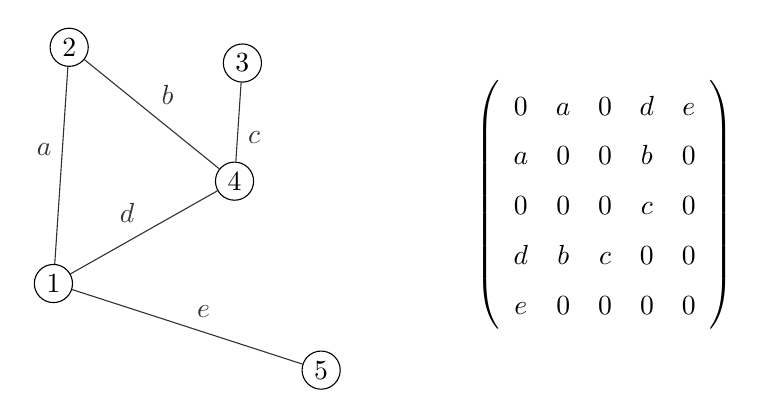
\begin{tikzpicture}[auto]
      \tikzstyle{every node} = [draw, circle, inner sep = 2pt]
      \node(1) at (1,2) {1};
      \node(2) at (1.2,5) {2};
      \node(3) at (3.4,4.8) {3};
      \node(4) at (3.3,3.3) {4};
      \node(5) at (4.4,0.9) {5};

      \tikzstyle{every node} = []
      \path[opacity=0.8]
      (1) edge node {$a$} (2);
      \path[opacity=0.8]
      (2) edge node {$b$} (4);
      \path[opacity=0.8]
      (4) edge node[swap] {$c$} (3);
      \path[opacity=0.8]
      (1) edge node {$d$} (4);
      \path[opacity=0.8]
      (1) edge node {$e$} (5);
      \node at (8,3) {$\left(\begin{array}{ccccc}
          0 & a & 0 & d & e\\
          a & 0 & 0 & b & 0\\
          0 & 0 & 0 & c & 0\\
          d & b & c & 0 & 0\\
          e & 0 & 0 & 0 & 0
        \end{array}\right)$};
    \end{tikzpicture}
  \end{center}
\caption{Example of a graph and its adjacency matrix}
\label{fig:graph}
\end{figure}

The \emph{order} of $G$ is equal to its number of vertices, possibly infinite.
The \emph{degree} of a vertex $v$ is equal to the number of edges it is attached to.
For digraphs the degree is the sum of the \emph{in}- and \emph{out}-degrees.
The \emph{degree} of $G$ refers to its max degree.
$G$ is said to be \emph{degree-regular} if all its vertices have the same degree.
If it is finite, its \emph{degree matrix} $D$ (\wrt to a vertex ordering $V = \{v_1, \ldots, v_n\}$) is the diagonal matrix for which the diagonal entry corresponding to a vertex is the sum of the weights of the edges it is part of.
Its \emph{laplacian matrix} $L$ is the substraction $L = D-A$, which can be \emph{normalized} $L = I - D^{-\frac{1}2}AD^{-\frac{1}2}$, \emph{left-normalized} $L = I - D^{-1}A$, or \emph{right-normalized} $L = I - AD^{-1}$. The same naming convention is used for normalized version of the adjacency matrix $A$.
A subgraph of $G$ induced by a subset $U \subset V$ is the graph with vertex and edge set restricted by $U$. The \emph{complement} graph $G^C$ shares the same vertex set but $u \overset{G^C}\sim v \Leftrightarrow u \overset{G}\nsim v$.
A \emph{complete} graph is such that there exists an edge between any two vertices.

\begin{definition}\textbf{Grid graph}\\
Let a graph $\gve$ such that the expression $u \sim v \Leftrightarrow \|u-v\|_1 = 1$ makes sense. $G$ can be called:
\begin{itemize}[nolistsep,noitemsep]
\item a \emph{grid graph} if $V = \bbz^2$
\item a \emph{finite grid graph} if $\exists (n,m) \in \bbz^2, V = \llbracket 1, n \rrbracket \times \llbracket 1, m \rrbracket$
\item a \emph{circulant grid graph} if $\exists (n,m) \in \bbz^2, V = \bbz /n \bbz \times \bbz /m \bbz$
\end{itemize}
\end{definition}

\begin{definition}\textbf{Bipartite graph}\\
A graph is called \emph{bipartite} if its vertex set is a disjoint union $V = V_1 \cup V_2$ \st $$u \sim v \Rightarrow (u,v) \in V_1 \times V_2 \vee (u,v) \in V_2 \times V_1$$
\end{definition}

If it is finite, its \emph{bipartite-adjacency} matrix $A \in \bbr^{V_1 \times V_2}$ is a rectangular matrix defined \wrt to a vertex ordering $V_1 = \{u_1, \ldots, u_n\}$, $V_2 = \{v_1, \ldots, v_n\}$ and weight mapping $w$ as $A[i,j] = w(u_i,v_j)$.

\begin{definition}\textbf{Signal}\\
A \emph{signal} on $V$, $s \in \cs(V)$, is a function $s: V \rightarrow \bbr$.
The \emph{signal space} $\cs(V)$ is the linear space of signals on $V$.
\end{definition}

\begin{remark}
In particular, a vector space, and more generally a tensor space, are finite-dimensional signal spaces on any of their bases. Reciprocally, a signal space is a linear space which canonical basis is the signal space domain. Therefore, signals can be represented as vectors (or tensors) and then fed to neural networks.
\end{remark}

A \emph{graph signal} on a graph $\gve$ is a signal on its vertex set $V$. We denote by $\cs(G)$ or $\cs(V)$ the graph signal space. $G$ can be referred as the \emph{underlying structure} of $\cs(V)$.
An \emph{entry} of a signal $s$ is an image by $s$ of some $v \in V$ and we denote $s[v]$. If~$v$~is represented by an $n$-tuple, we can also write $s[v_1, v_2, \ldots, v_n]$.
The \emph{support} of a signal $s \in \cs(V)$ is the subset $\supp(s) \subset V$ on which $s \neq 0$.
For spaces of signals that aren't real-valued, their codomain~$\bbe$ is precised in the subscript~$\cs_{\bbe}(V)$.
The signal $\id$ is the identity function.
Given $v \in V$, the dirac signal $\delta_v \in \cs(V)$ is the signal valued as $1$ on $v$ and $0$ everywhere else. The family of all dirac signals spans~$\cs(V)$.

\subsection{Learning tasks}

There are two main tasks related to deep learning and graph signals.

\paragraph{Supervised classification of graph signals}
This is the classical application of deep learning transposed to graph signals, rather than image or audio signals. It is the main task we will have in mind in the course of this manuscript. Given a graph $\gve$ and an input signal $x \in \cs(G)$ the goal is to classify~$x$. If there are~$c$ possible classes, a neural network~$f$ outputs a vector $y = f(x)$ of dimension~$c$, and its dimension with the biggest weight determines the predicted class. Indeed, a standard MLP can be trained on a dataset of graph signals. However, an MLP wouldn't take the graph structure $G$ into consideration. By similarity with CNNs that leverage the grid structure of images to achieve better performances than MLPs, a challenge is to define a neural network on graph signals that can leverage~$G$. We review some models from the literature in \secref{sec:spec} and in \secref{sec:vert}. We develop an algebraic understanding in \chapref{chap:2} of why and how they should work, and also propose our own models and point of view in \chapref{chap:3}.

\paragraph{Semi-supervised classification of nodes}
This task is in some way obtained from a transposed perspective of the previous one. Given a dataset of graph signals, represented as a matrix $X \in \bbr^{n \times N}$, where the rows represent the nodes, and the columns represent the signals, the goal is to classify the nodes. This amounts to classify the rows, whereas the previous task amounts to classify the columns. As opposed to the previous one, this task is \emph{transductive} \ie every node data is available during training, including those from the validation and test set (but their labels are not), and it is \emph{semi-supervised} \ie some nodes have no label. This allows to learn on much more data than if we were restricted to labeled data. In this task, the edges connect learning samples, however in the previous one, the edges were connecting features of learning samples. This is this edge relationship between learning samples that renders the semi-supervised approach possible. This task have received much more attention than the previous one in the recent literature. We explain why in \secref{sec:spec}.

\paragraph{Other learning tasks}
In this manuscipt, we are less interested in other deep learning tasks related to graphs, so we briefly discuss them here. One is supervised classification of graphs, which is different than classifying graph signals. Examples include \citep{niepert2016learning,tixier2017classifying,nikolentzos2017kernel,bai2018quantum}. Another related interesting task is called representation learning of nodes, which tackles the challenge to learn a linear representation of nodes. A common approach, derived from word2vec \citep{mikolov2013efficient,mikolov2013distributed}, is called node2vec \citep{grover2016node2vec}, and was later improved in graphSAGE \citep{hamilton2017inductive}. A review on this subject is done by \cite{hamilton2017representation}. A thorough survey on representation learning for networks is given in \citep{zhang2017network}.

\subsection{Datasets}
\label{sec:datasets}

We present here the standard datasets that we will use in this manuscript.

\paragraph{Images}
Images are signals on grid graphs. Therefore they constitute a first test for models that are designed to be able to classify graph signals. A second step is to test on scrambled versions of image datasets, \ie a random permutation of the pixels is fixed and the tested models are fed with images whose pixels have been shuffled according to this permutation.
Therefore the domains of the scrambled input signals are not grid graphs.
\begin{itemize}
  \item MNIST~\citep{lecun1998mnist} is a dataset of handwritten digits of size 28x28. It contains 10 classes and is splitted between 50'000 samples for training and 10'000 samples for testing.
  \item CIFAR-$10$~\citep{krizhevsky2009learning} is a dataset of tiny pictures of size 32x32. It contains 10 classes and is splitted between 50'000 samples for traning and 10'000 samples for testing.
  \item Scrambled MNIST is the scrambled version of MNIST. A graph based on nearest neighbours from the pixel covariances is used to represent each scrambled sample as a graph signal.
  \item Scrambled CIFAR-$10$ is analoguous.
\end{itemize}

\paragraph{Functional magnetic resonance imagings (fMRI)}
fMRI samples can be represented by graph signals. The graphs are resembling grid graphs to some extent since they are embedded in an Euclidean space.
\begin{itemize}
  \item The PINES dataset consists of fMRI scans on 182 subjects, during an emotional picture rating task \citep{chang2015sensitive}. In \citep{lassance2018matching}, we fetched individual first-level statistical maps (beta images) for the minimal and maximal ratings from \url{https://neurovault.org/collections/1964/}, to generate the dataset. Full brain data was masked on the MNI template and resampled to a 16mm cubic grid, in order to reduce dimensionality of the dataset while keeping a regular geometrical structure to infer the graph. Final volumes used for classification contain 369 signals for each subject and rating.
\end{itemize}

\paragraph{Text documents}
Text documents can be represented as graph signals. Words are the vertices, and the value of a signal at a given vertex corresponds to a normalized occurence of the corresponding word. Edges connect nearest neighbours in some metric space.
\begin{itemize}
  \item $20$NEWS \citep{joachims1996probabilistic} is a dataset of text documents. It contains 20 classes and is splitted between 11'314 samples for training and 7'532 samples for testing. Each document is represented by a bag-of-word. In the version used by \cite{defferrard2016convolutional}, that we consider, documents are treated as signals on a graph of 10'000 vertices which represent the 10'000 most common words (the other words are not used). Edges are drawn from each vertex to their 16 nearest neighbours in the cosine similarity metric space.
\end{itemize}

\paragraph{Citation networks}
In a citation network (\ie a graph of citations), nodes are bag-of-word documents and edges represent citations. Models are tested on a citation network to the task of semi-supervised classification of the nodes. We use three standard datasets: Cora, Citeseer and Pubmed~\citep{sen2008collective}, for which we follow the experimental settings of \cite{yang2016revisiting}, and the dataset split from \cite{kipf2016semi}. In particular, there are only 20 training samples per class, but they are connected to other samples.
\begin{itemize}
  \item Cora is a dataset of 2'708 nodes of dimension 1'433 with 5'429 edges. It contains 7 classes and consists of 140 samples for training, 500 samples for validation, 1'000 samples for testing, and 1'068 unlabelled samples.
  \item Citeseer is a dataset of 3'327 nodes of dimension 3'703 with 4'732 edges. It contains 6 classes and consists of 120 samples for training, 500 samples for validation, 1000 samples for testing, and 1'707 unlabelled samples.
  \item Pubmed is a dataset of 19'717 nodes of dimension 500 with 44'338 edges. It contains 3 classes and consists of 60 samples for training, 500 samples for validation, 1000 samples for testing, and 18'157 unlabelled samples.
\end{itemize}


\subsection{Spectral methods}
\label{sec:spec}

Spectral methods are based on spectral graph theory \citep{chung1996spectral} which aims at characterizing structral properties of a graph $\gve$ through the eigenvalues of the laplacian matrix $L$. In particular, since it is hermitian, it admits a complete set of normalized eigenvectors. By fixing a normalized eigenvector basis ordered in the rows of $U$ (by ascending eigenvalues), $U$ is used to define the \emph{Graph Fourier Transform} (GFT) of a signal $s \in \cs(G)$ \citep{shuman2013emerging}, and the conjugate-transpose $U^*$ defines the inverse GFT. We write
\begin{align}
\widehat{s} &= Us\\
\widetilde{s} &= U^*s
\end{align}

\begin{remark}
The GFT extends the notion of \emph{Discrete Fourier Transform} (DFT) to general graphs, since that for circulant grid graphs $U$ can be the DFT matrix.
\end{remark}

By analogy with the convolution theorem, a convolution can be defined as pointwise multiplication, denoted $\cdot$, in the spectral domain of the graph \citep{hammond2011wavelets}. For $s, g \in \cs(G)$, we have:
\begin{gather}
s \ast g = \widetilde{\widehat{s} \cdot \widehat{g}} \label{eq:sc}
\end{gather}

This expression can be used to define convolutional layers and spectral CNNs on graphs. However, \cite{bruna2013spectral} pointed out that \eqref{eq:sc} would generate filters with $\co(n)$ weights, where $n$ is the order of $G$. So they proposed to learn filters $\theta$ with only $\co(1)$ weights and then to smoothly interpolate the remaining weights as $g = K \theta$, where $K$ is a linear smoother matrix. They motivate their construction by the fact that smooth multipliers in the spectral domain should simulate local operations in the vertex domain. To elaborate a bit on this, note that we have:
\begin{align}
Ls[u] &= \displaystyle\sum_{v \in V} w(u,v)(s[u] - s[v])
\end{align}
And so,
\begin{align}
s^TLs &= \displaystyle\sum_{u \in V}\sum_{v \in V} w(u,v)s[u](s[u] - s[v])\nonumber\\
&= \displaystyle \frac{1}2\sum_{u \in V}\sum_{v \in V} w(u,v)s[u](s[u] - s[v]) + \frac{1}2\sum_{v \in V}\sum_{u \in V} w(v,u)s[v](s[v] - s[u])\nonumber\\
&=  \displaystyle\sum_{u \in V}\sum_{v \in V} \frac{w(u,v)}2(s[u] - s[v])^2 \label{eq:smooth}
\end{align}
That is, $s^TLs$ is some sort of measure of \emph{smoothness} of the signal $s$, penalized by the weights $w$. The bigger is $w(u,v)$, the closest $s(u)$ and $s(v)$ must be to lower the smoothness \eqref{eq:smooth}. Since $L$ is symmetric, its eigenvalues are non-negative real numbers, and $U$ diagonalizes $L$ as $\Lambda = ULU^*$. Denote $(\lambda_i)_i$ the eigenvalues, the smoothness measure rewrites:
\begin{align}
s^TLs = \widehat{s}^*\Lambda\widehat{s} = \displaystyle\sum_{i=1}^n \lambda_i \widehat{s}[i]^2
\end{align}
Therefore, as they pointed out, smoothness of~$s$ can be read off the coordinates of~$\hat{s}$, like for the DFT. Moreover, spectral multipliers modulate its smoothness, and decay in the spectral domain is related to smoothness in the vertex domain. But contrary to their conjecture, smoothness in the spectral domain is not necessary related to decay is the vertex domain (and so to some form of locality). For instance, since the laplacian~$L^C$ of the complement graph~$G^C$ commutes with~$L$, it can share the same eigenvector basis~$U$, and thus define the same GFT, but their notion of locality in the vertex domain are opposed. Another drawback is that this method requires computing the GFT which complexity is at least~$\co(n^2)$ as there is no equivalent of the Fast Fourier Transform (FFT) on graphs, so the authors suggest to use a lower number of eigenvectors $d < n$ from the laplacian eigenbasis.

Then, \cite{defferrard2016convolutional} remedy to these issues by proposing an approximate formulation based on the Chebychev polynomials, denoted by $(T_i)_i$, where $i$ is the polynomial order.
That is, their proposed approximate filters are in the form
\begin{gather}
g_\theta(L) = \sum_{i=0}^k \theta[i] \h{2} T_i(\widetilde{L}) \label{eq:cheb}
\end{gather}
where $\widetilde{L} = \frac{\lambda_{\max}}2L - I_n$ is the scaled normalized laplacian with eigenvalues lying in the range $[-1,1]$. $g_\theta(L)$ are spectral multipliers since we have:
\begin{align}
g_\theta(L)s &= g_\theta(U^*\Lambda U)s
= U^* g_\theta(\Lambda) Us\nonumber\\
&= \widetilde{g_\theta(\Lambda) \mathbf1} \ast s
\end{align}

These filters enjoy locality properties, they contain~$\co(1)$ weights, and their complexity is~$\co(n)$ when rows of~$L$ are sparse. The use of truncated Chebychev expansion \citep{hammond2011wavelets} ensures that in theory any set of spectral multipliers can be approximated. Also, since they are laplacian polynomials, some authors would argue that these filters are transferable from one graph to another. From a combinatorial point of view this is true. However there is no reason that spectral multipliers from a spectral domain make sense in another one, and there are no experiment in the literature to support the hypothesis. On the other hand, \citep{yi2016syncspeccnn} (who do not use polynomial filters) fix a canonical spectral base in order to synchronize every spectral domains. Their idea is to learn a warping from any eigenbasis to the canonical one, prior to performing spectral multiplication, in the manner of spatial transformer networks (STN, \cite{jaderberg2015spatial}).

However, it is hard to evaluate if a model performs well on the task of supervised classification of graph signals, because there are not much known datasets in the literature for which the given graph domain holds enough information.

For example, \citeauthor{defferrard2016convolutional} built a graph signal dataset from the text categorization dataset $20$NEWS (\cite{joachims1996probabilistic}, see \secref{sec:datasets}). However, their model (ChebNet32) fails to surpass Multinomial Naive Bayes (MNB). Moreover, even though they report that their model beats MLPs, but through experiments we noticed the contrary. In results we report in \tabref{tab:20}, we see that a lighter MLP, composed of a single Fully-Connected~(FC) layer with ReLU and 20\% dropout outperforms ChebNet32. We replicated their preprocessing phase from the code on their official repository and averaged our results on 100 runs of 10 epochs\footnote{A few epochs are enough since models seem to overfit fast on this dataset.}.

\begin{table}[H]
  \caption{Accuracies (in \%) on $20$NEWS}
  \begin{center}
    \bgroup
    \def\arraystretch{1.5}%  1 is the default, change whatever you need
    \begin{tabular}{|c|c|c|c|c|}
      \hline
      MNB & FC2500 & FC2500-FC500 & ChebNet32 & FC500\\
      \hline
      $68.51^a$ & $64.64^a$ & $65.76^a$ & $68.26^a$ & $\mathbf{71.96} \pm 0.15^b$\\
      \hline
    \end{tabular}
    \egroup
  \end{center}
\begin{flushleft}
\footnotesize{
$^a$ As reported in \cite{defferrard2016convolutional}\\
$^b$ From our experiments.
}
\end{flushleft}
  \label{tab:20}
\end{table}

Despite the significant theoretical contribution, this negative result stresses out the importance of the graph used in practice to support the convolution, a point that they also discussed. \cite{henaff2015deep}, proposed supervised graph estimation techniques, but a better graph signal dataset would be one that come with an already suitable graph, that of current literature is still lacking.

On the other hand, attention in the domain has shifted toward the task of semi-supervised classification of nodes, where good datasets are not lacking. For example, \cite{levie2017cayleynets}, mainly demonstrate the usefulness of their model on these type of tasks. They define polynomial filters, for which Chebychev filters are a special case, that are capable to specialize in narrow bands of frequency in the spectral domain.

Another spectral avenue consists in using wavelets defined in the graph spectral domain \citep{hammond2011wavelets}, in order to build a scattering network \citep{bruna2013invariant,chen2014unsupervised}. This idea have been exploited recently by \cite{zou2018Graph}, then by \cite{gama2018Diffusion}.

\subsection{Vertex-domain methods}
\label{sec:vert}

As their name suggests, vertex-domain methods operates directly on the vertices of the graph. % These works were originally motivated by chemistry datasets~\citep{duvenaud2015convolutional,kearnes2016molecular}.
Convolution can be modelized as a function $f$ of the kernel weights $\theta$ and neighboring vertices (contained in the local receptive field $\ccr(v)$), usually based on dot products. That is
\begin{gather}
y[v] = f_\theta\left(\{u \in \ccr(v)\}\right)
\end{gather}
As such, it retains the property of being localized and of sharing weights in some way. But there remains the need to specify how the shared weights are allocated in this local receptive field~\citep{vialatte2016generalizing}. This allocation can depend on \eg an arbitrary order~\citep{niepert2016learning}, on a diffusion process~\citep{atwood2016diffusion}, on a function of both vertices and their neighbors~\citep{monti2016geometric,simonovsky2017dynamic}, on a random walk \citep{hechtlinger2017generalization}, on another learned kernel~\citep{vialatte2017learning}, on an attention mechanism~\citep{velickovic2017graph,lee2018attention}, on pattern identification~\citep{sankar2017motif}, or on translation identification~\citep{pasdeloup2017convolutional}. All these methods differ in the function~$f$, but in the end, their definition highly overlap. That is why some authors have proposed unified frameworks~\citep{gilmer2017neural}. The representation we present in \chapref{chap:3} is also unifying in that sense (see \secref{sec:gen}).

In particular, \cite{kipf2016semi}, were first to transpose ChebNet to the task of semi-supervised node classification. Chebychev filters \eqref{eq:cheb} then take a form that is interpretable in the vertex domain, which is
\begin{gather}
Y = \displaystyle\sum_{i=0}^k T_i(\widetilde{L}) X \Theta
\end{gather}
where $X \in \bbr^{n \times N}$, $\Theta \in \bbr^{N \times M}$, $n$ is the number of nodes, $N$ is the number of input channels (features per node), and $M$ is the number of output feature maps. On the left, powers of $\widetilde{L}$ diffuse the graph signal $X$ to share node information. On the right, $\Theta$ maps the diffused signals to another representation. So in essence, this formulation is more a vertex-domain method. They found that the best performing filters were expressed in a simplified form
\begin{gather}
Y = \widetilde{A} X \Theta \label{eq:gcn}
\end{gather}
where $\widetilde{A}$ is the normalized adjacency matrix of the graph to which self-loops are added. They call the architecture composed with these filters a Graph Convolution Network (GCN). Similiarly, $\widetilde{A}X$ shares node information via the edges and $\Theta$ makes the model learns. This fomulation attracted a lot of research attention and was, in particular, extended with attention mechanism (no pun intended), inspired from the field of neural machine translation \citep{bahdanau2014neural}. A review is done by \cite{lee2018attention}.

For example, \cite{velickovic2017graph}, propose a model that learns attention in a local receptive field. They call it Graph ATtention network (GAT). The attention mechanism is parameterized by a neural network $a$, containing a single FC layer $(g,\text{LeakyReLU})$, which takes as input a couple of neighboring nodes $(i,j)$ and outputs a scalar $\alpha_{i,j}$. The attention that $i$ deserves to $j$ is:
\begin{gather}
\alpha_{i,j} = \text{softmax}_j\left(a( X[i,:] \h{2} \Theta \h{2} \mathbin{\|} \h{2} X[j,:] \h{2} \Theta )\right)
\end{gather}
where $\mathbin{\|}$ denotes concatenation. In a sense, $a$ learns which input feature maps are most useful to describe the attention a node should derserve to another. The forward propagation is done similarly than \eqref{eq:gcn}, but with a matrix $A_k$ filled with the attention coefficients $\alpha_{i,j}$ instead of $\widetilde{A}$. They also propose that the model learns multiple attention heads, so that a GAT layer amounts to:
\begin{align}
Y &= \displaystyle\bigparallel_{k=1}^K A_k X \Theta_k\\
\text{or } Y &= \frac{1}K\displaystyle\sum_{k=1}^K A_k X \Theta_k
\end{align}

Another method called Topology Adaptative GCN (TAGCN, \cite{du2017topology}) uses a convolution filter borrowed from graph signal processing literature~\citep{sandryhaila2013discrete}, which is defined in the vertex domain as:
\begin{gather}
Y[:,f] = \sum_{c = 1}^N \left(\sum_{k=1}^K \Theta_k[c,f] \h{2} \widetilde{A}^k \right) X[:,c]
\end{gather}
It can be rewritten as:
\begin{gather}
Y = \sum_{k=1}^K \widetilde{A}^k X \Theta_k
\end{gather}
Each succesive powers of the normalized adjacency matrix $\widetilde{A}$ allows for considering wider neighborhoods.

Other works extending or resembling GCN are numerous in recent days (\eg \cite{niepert2018towards}). We do not cover them since that their novelty compared to GCN is limited.

\paragraph{\h{0}}
In the next chapter, we study how to characterize a convolution of graph signals in the vertex domain.